\section{设计}\label{sec:design}

\subsection{概述}
本节简要概述Fidelius中使用的enclaves和符号,以及其架构和工作流程。

\begin{figure*}[h]
\centering
\hspace*{-0.5cm}
\scalebox{.45}{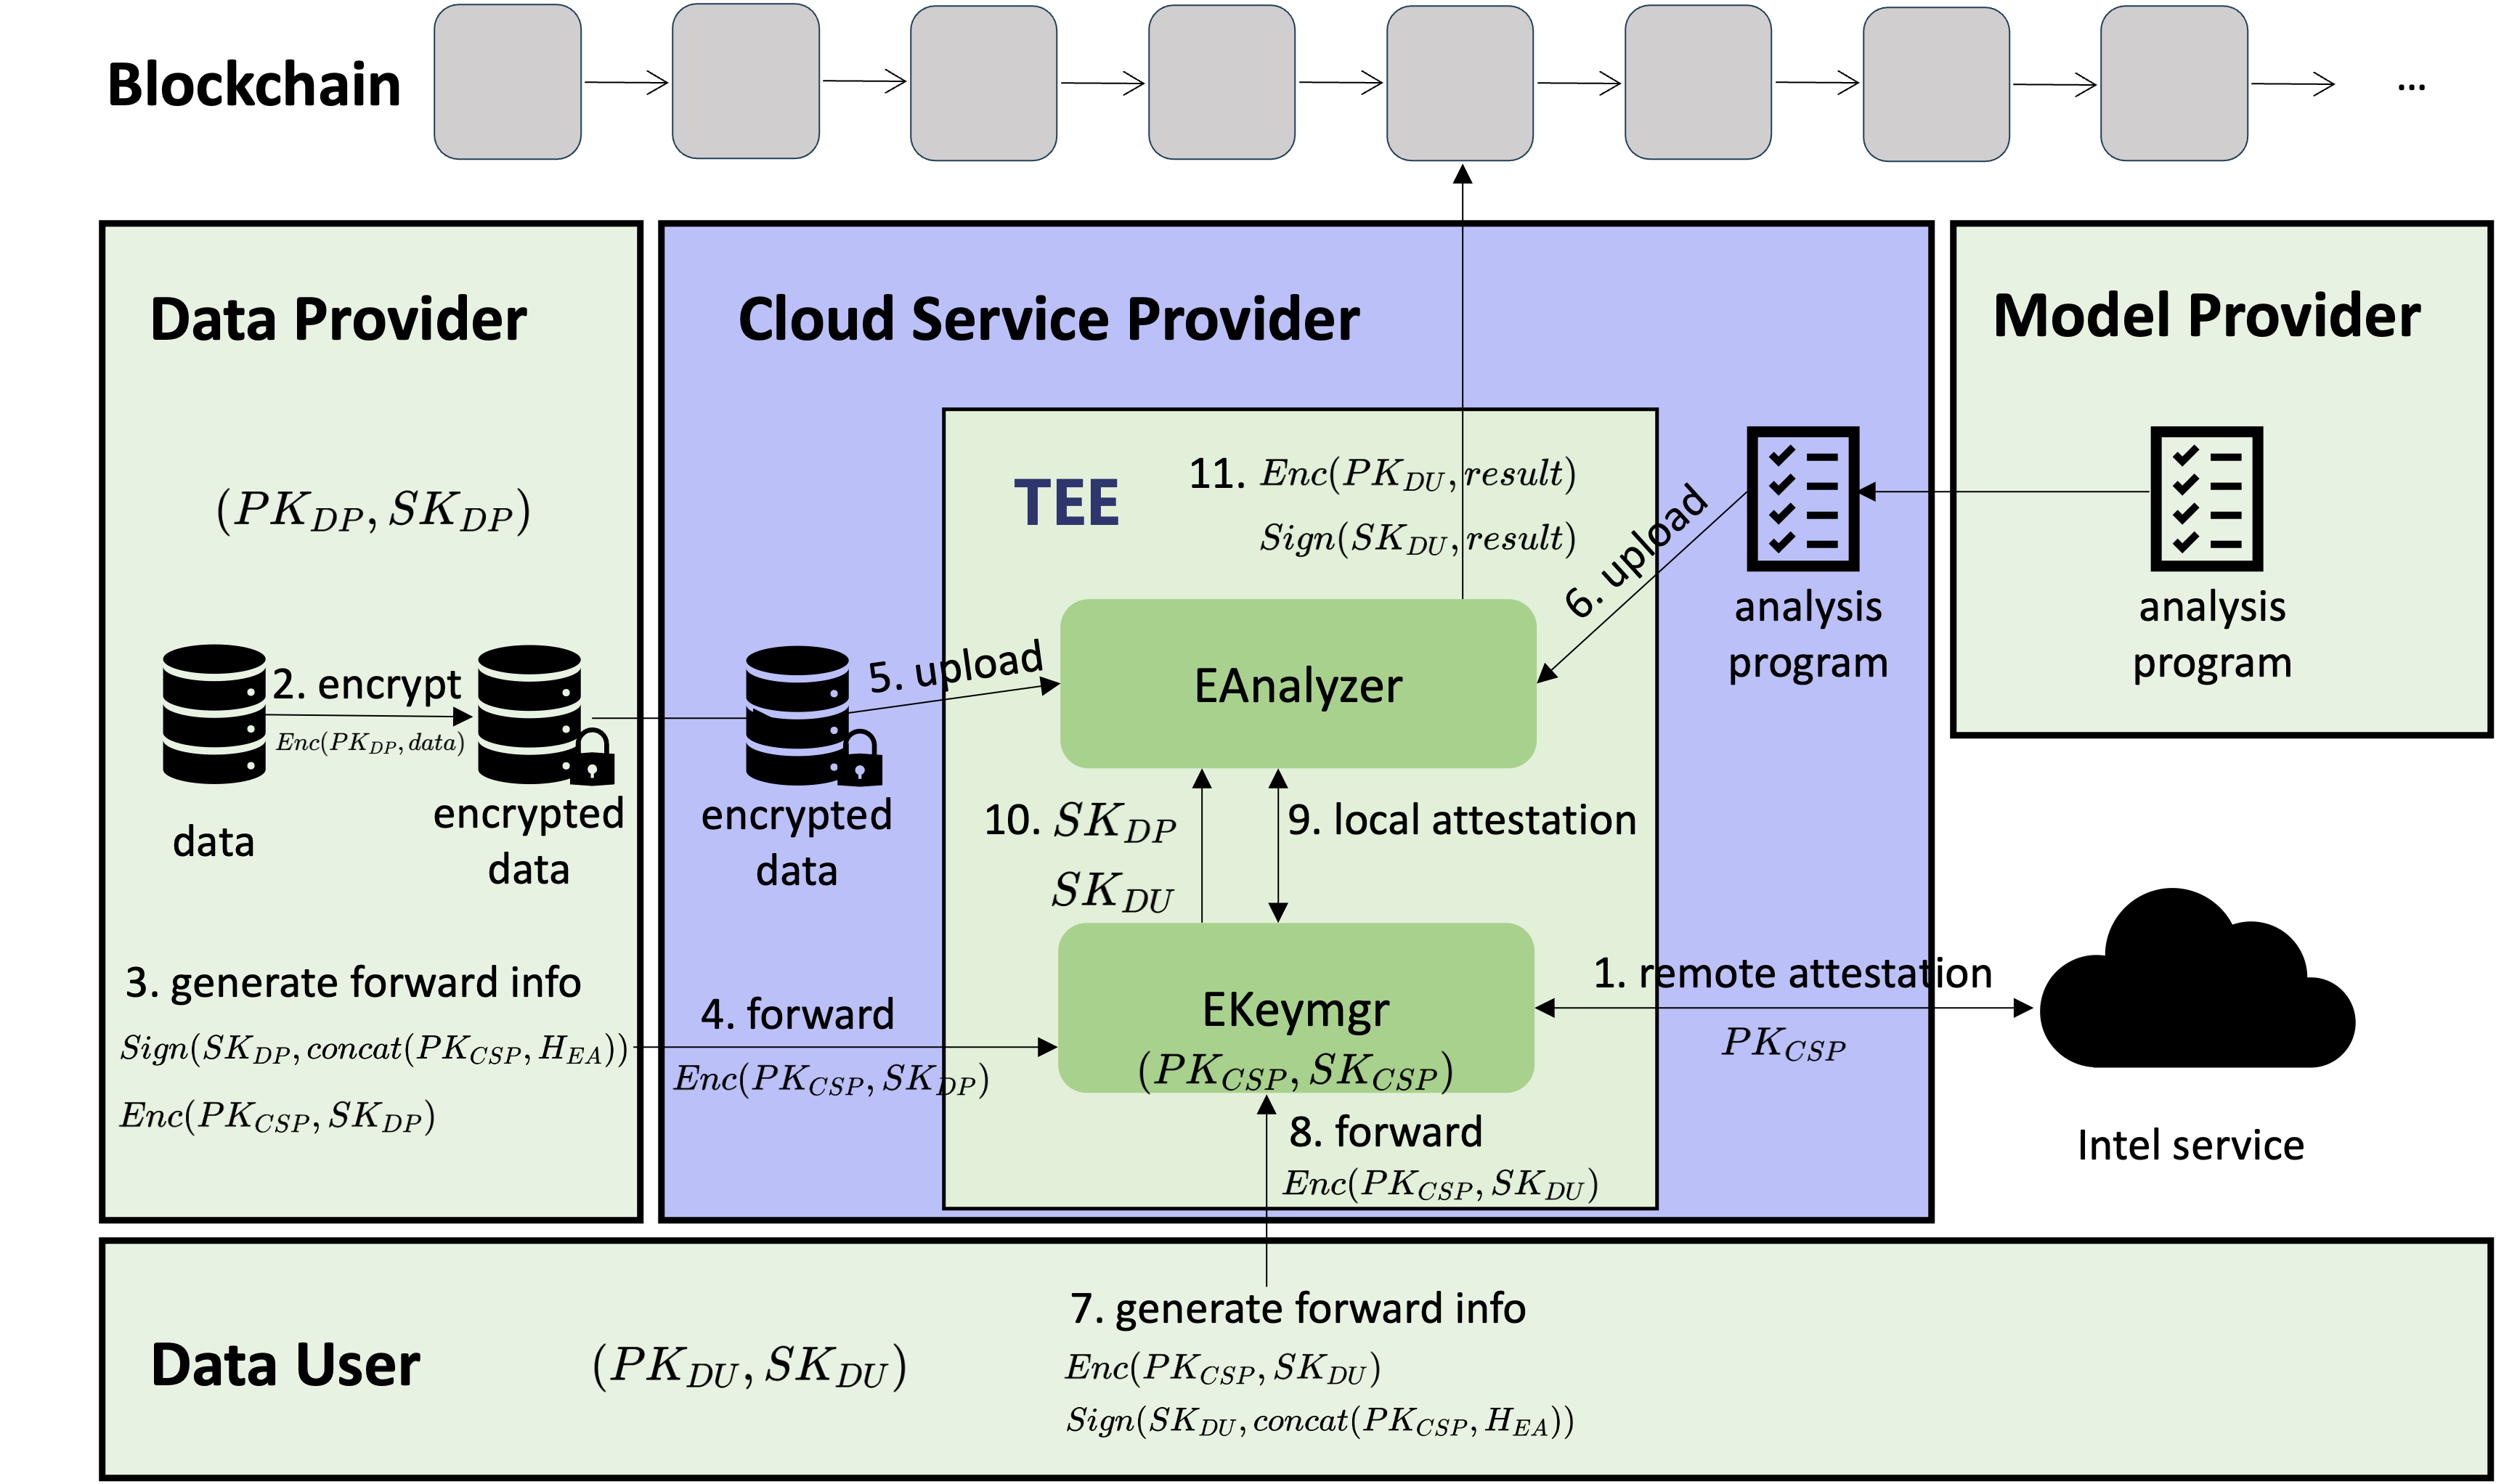
\includegraphics{images/architecture.png}}
  \caption{\small 数据分析架构和工作流程。}
  \label{fig:arch}
\end{figure*} 
\subsubsection{Enclaves和符号}
在本文中,我们定义以下enclaves和符号:
\begin{itemize}
    \item EKeyMgr。Enclave密钥管理器管理非对称密钥,处理创建、删除并提供基本密码学功能,包括消息加密、解密、签名和签名验证。
    \item EAnalyzer。Enclave分析器,一个Intel SGX Enclave格式的分析程序,确保程序在执行期间保持不变。
    \item $(PK_{DP},SK_{DP})$,数据提供方的非对称密钥对。
    \item $(PK_{DU},SK_{DU})$,数据使用方的非对称密钥对。
    \item $(PK_{CSP}, SK_{CSP})$表示云服务提供方的非对称密钥对,由EKeyMgr生成。私钥$SK_{CSP}$安全地存储在enclave内,确保云服务提供商无法提取。
    \item $H(\cdot)$表示哈希函数。
    \item $Enc(PK, msg)$表示使用$PK$加密$msg$。
    \item $Dec(SK, cipher)$表示使用$SK$解密$cipher$。
    \item $Sign(SK, msg)$表示使用$SK$对$msg$进行签名。
    \item $Verf(PK, msg, sig)$表示使用$PK$和$msg$验证$sig$。
    \item $\digamma(SK, PK_{CSP}, H_{EA})$表示使用$PK_{CSP}$将$SK$转发到EKeyMgr的过程。在此上下文中,$SK$在EAnalyzer中使用,由$H_{EA}$标识。函数$\digamma(\cdot)$涉及$Sign(SK, concat(PK_{CSP}, H_{EA}))$和$Enc(PK_{CSP}, SK)$。
\end{itemize}

\subsubsection{架构和工作流程}

Fidelius架构和数据分析工作流程如图~\ref{fig:arch}所示。
该过程从设置阶段开始,其中CSP中的EKeyMgr生成非对称密钥对。公钥$PK_{CSP}$通过Intel的远程认证服务进行验证,而私钥$SK_{CSP}$安全地存储在EKeyMgr内。同时,数据提供方(DP)和数据使用方(DU)各自生成自己的非对称密钥对,并保留这些密钥。此外,DP使用她的公钥$PK_{DP}$加密数据,并为DU的使用准备这些加密数据。

DP将加密数据上传到CSP,并使用$\digamma(SK_{DP}, PK_{CSP}, H_{EA})$将她的私钥$SK_{DP}$转发给EKeyMgr。类似地,DU将分析程序上传到CSP,并使用相同的方法将她的私钥$SK_{DU}$转发给EKeyMgr。重要的是要注意,明文私钥($SK_{DP}$和$SK_{DU}$)只能在EKeyMgr内解密。

一旦分析程序、加密数据和私钥准备就绪,数据分析任务就开始了。首先根据隐私描述语言(PDL)定义的规则检查分析程序。任何未通过此检查的程序都会导致分析任务立即终止。随后,EAnalyzer加载并解密加密数据。然后验证解密数据的哈希值;如果与声称的哈希不匹配,EAnalyzer立即停止以防止处理被篡改或欺诈的数据。如果数据得到验证,EAnalyzer继续进行主要分析,最终使用$PK_{DU}$产生加密结果。此外,使用$SK_{DU}$对结果进行签名。由于$SK_{DU}$位于EKeyMgr内,EAnalyzer通过本地认证建立安全通道来请求$SK_{DU}$。

\begin{figure}[h]
\centering
\begin{lstlisting}
import number;
in = input user_type_t;
iris = in.iris_data;
sum(s1, s2) = {data: s1.data + s2.data, 
    counter: s1.counter + s2.counter}
sl = {data: iris.sepal_len, counter:number.one} |
     sum(sl:s1, sl:s2);
sw = {data:iris.sepal_wid, counter:number.one} |
     sum(sw:s1, sw:s2) ;
pl = {data:iris.petal_len, counter:number.one} |
     sum(pl:s1, pl:s2) ;
pw = {data:iris.petal_wid, counter:number.one} |
     sum(pw:s1, pw:s2) ;
osl = sl.data/sl.counter;
osw = sw.data/sw.counter;
opl = pl.data/pl.counter;
opw = pw.data/pw.counter;
output osl, osw, opl, opw, in.species
\end{lstlisting}
\caption{使用PDL授权Iris数据集上的KMeans算法}
\label{fig:pdl}
\end{figure} 
\subsection{隐私描述语言}
% 为了防止数据分析结果泄漏数据,我们提出了隐私描述语言来定义使用数据的规则,并通过了静态⼆进制分析的⽅法检查分析程序是否遵守隐私描述语言定义的规则。如图所示,这段代码使用PDL描述了在Iris数据集上使用Kmeans算法的规则,这段代码也将被转换成LLVM的中间表示,然后使用符号执行得到PDL描述的规则的状态a。另一方面,我们使用GTIRB作为分析的中间表⽰,在将分析程序转换为中间表⽰后,使⽤符号执⾏获取每个输出变量的状态b,并判断是否满足b包含于a。
为了防止分析结果中的数据泄露,我们开发了一种隐私描述语言(PDL)来定义数据使用规则。使用静态二进制分析来确保分析程序遵循这些PDL定义的规则。如图~\ref{fig:pdl}所示,代码片段使用PDL来指定在Iris数据集上应用KMeans算法的规则。然后将此代码转换为LLVM的中间表示(IR),接着进行符号执行~\cite{king1976symbolic,baldoni2018survey}以得出PDL描述的状态$S$。同时,我们在分析中使用GTIRB~\cite{schulte2019gtirb}作为中间表示。将分析程序转换为此格式后,应用符号执行来获得每个输出变量的状态$S^{\prime}$,确保$S^{\prime}$是$S$的子集,从而确认合规性。

\subsection{可信和可验证的结果}
算法~\ref{algo:analysis_enclave}概述了EKeyMgr和EAnalyzer的主要操作。在EAnalyzer内生成的加密分析结果及其签名被传输到区块链。在那里,任何人都可以验证签名的有效性。有效的签名确认DP成功执行了分析程序并获得了正确的结果,因为签名源自EAnalyzer内部。这种机制防止攻击者在未执行分析程序的情况下伪造有效签名,从而确保数据分析过程的完整性。DU可以从区块链下载加密结果,并使用$SK_{DU}$解密以获得明文分析结果。
\SetKwInput{KwThrow}{throw}
\begin{algorithm}[h]
  \caption{Enclave密钥管理器和分析器}
  \KwIn{$Enc_{SK_{DP}}$, $Enc_{SK_{DU}}$, $Sig$, $Enc_{data}$, data\_hash, $H_{EA}$}

  \tcc{EKeyMgr - 密钥管理阶段}
  $SK_{DP} \gets Dec(SK_{CSP},Enc_{SK_{DP}})$\;
  $SK_{DU} \gets Dec(SK_{CSP},Enc_{SK_{DU}})$\;
  \If{$!Verf(PK_{CSP}, concat(SK_{DP}, SK_{DU}), Sig)$}{\KwThrow{``密钥验证失败'';}}

  \tcc{EAnalyzer - 分析执行阶段}
  $PK_{DU} \gets generate\_pkey\_from\_skey(SK_{DU})$\;
  $enclave\_hash \gets get\_current\_enclave\_hash()$\;
  \If{$enclave\_hash \ne H_{EA}$}{\KwThrow{``Enclave完整性验证失败'';}}
  \If{$!Verf(PK_{DU},concat(PK_{CSP},enclave\_hash),Sig)$}{\KwThrow{``无效的EAnalyzer'';}}
  
  $data \gets Dec(SK_{DP},Enc_{data})$\;
  \If{$H(data) \ne data\_hash$}{\KwThrow{``数据完整性验证失败'';}}
  
  $result \gets do\_parse()$\;
  \If{$result == null$}{\KwThrow{``分析执行失败'';}}
  
  $Enc_{res} \gets Enc(PK_{DU},result)$\;
  $Sig_{res} \gets Sign(SK_{DU},concat(result, enclave\_hash))$\;
  
  \KwRet{$(Enc_{res}, Sig_{res})$ 并发送到区块链}\;
\label{algo:analysis_enclave}
\end{algorithm} 

\subsection{一次性远程认证}
%We implement a one-time remote attestation as outlined in Algorithm~\ref{algo:attestation}. 
我们实施一次性远程认证过程,如算法~\ref{algo:attestation}所述,从一开始就建立安全和可信的环境。 
%During the setup phase, the Cloud Service Provider (CSP) verifies the authorization of $PK_{CSP}$, generated by EKeyMgr, through a remote attestation with Intel service. 
在设置阶段,云服务提供商(CSP)通过与Intel认证服务进行远程认证来验证EKeyMgr生成的公钥$PK_{CSP}$的授权。这种彻底的验证确认了CSP凭据的完整性和合法性。
一旦验证完成,CSP上的后续分析任务不再需要远程认证。DP和DU转发的私钥($SK$)通过本地认证从EKeyMgr安全传输到EAnalyzer。
%We incorporate a one-time remote attestation process, as detailed in Algorithm \ref{algo:attestation}, to establish a secure and trusted environment from the outset. During the initial setup phase, the Cloud Service Provider (CSP) rigorously validates the authorization of the public key $PK_{CSP}$ generated by EKeyMgr by performing a remote attestation with Intel's attestation service. This thorough verification confirms both the integrity and legitimacy of the CSP's credentials. Once this attestation is successfully completed, all subsequent analysis tasks on the CSP can be executed without further attestation, thereby streamlining operations and reducing overhead. Additionally, the private keys ($SK$) supplied by the DP and DU are securely transmitted from EKeyMgr to EAnalyzer via a robust local attestation process, ensuring that sensitive cryptographic material remains confidential and tamper-resistant throughout the transfer. 